\chapter{Theoretical and optical analyses}
\label{chap:theoretical-optical-analyses}

This chapter establishes the theoretical and optical basis used to define the main design constraints of the LINKU stereo vision system. After identifying the need for a dedicated geometric reconstruction approach, the next step is to determine whether the tether can be visually observed and reconstructed under the expected orbital conditions.
\\\\
The analysis focuses on three principal design drivers, the dynamic behavior of the tethered formation, the optical field of view required to maintain visual coverage, and the geometric resolution needed to detect a thin tether over the expected separation range. These constraints define the trade-off between situational awareness during deployment and geometric accuracy during post-deployment characterization.

\section{Dynamic constraints and field of view estimation}

Understanding the expected motion of the tethered formation is a prerequisite for defining the camera field of view and preserving line-of-sight during the mission. The stereo vision system must be able to observe the tether during the deployment process, when the configuration may exhibit transient attitude motion, and during the post-deployment regime, when the tethered system is expected to evolve toward gravity-gradient stabilization.
\\\\
In this context, gravity-gradient stabilization refers to the tendency of the tether axis and the connected satellite masses to align approximately along the local orbital radial direction. In the Local Vertical Local Horizontal reference frame, this corresponds to the Nadir--Zenith axis, with Nadir pointing toward the Earth's center and Zenith pointing away from it. Therefore, the tethered configuration is expected to oscillate around this radial equilibrium direction rather than remain perfectly static.
\\\\
The physical origin of this behavior is the differential gravitational acceleration experienced along the length of the tethered system. The gravitational acceleration at a distance r from the Earth's center can be expressed as:

\begin{equation}
g(r) = \frac{\mu}{r^2}
\label{eq:gravity}
\end{equation}

where $\mu \approx 3.986 \times 10^{14}\ \mathrm{m^3\,s^{-2}}$ is Earth's standard gravitational parameter.
\\\\
Because the two tethered masses are located at slightly different radial distances from the Earth's center, they experience slightly different gravitational accelerations. This differential effect produces a restoring tendency that aligns the tethered system with the local radial direction and generates librational motion around the Nadir-Zenith axis.
\\\\
For the purpose of field-of-view estimation, the optical design must account for both deployment transients and the expected post-deployment oscillatory behavior. Dynamic trends identified in Deliverable D4 indicate that the tethered system response is sensitive to initial attitude deviations and to the relationship between body-angular and orbital-frame angular velocities. These simulations also suggest that out-of-plane deviations may induce cone-like motion around the Nadir direction, requiring additional angular margin in the optical design. A representative stable case considered in D4 includes initial pitch and roll deviations of approximately $10^\circ$.
\\\\
Since the final long-term stabilization envelope is still under definition, the field of view must be sized conservatively. The optical design should therefore accommodate expected librational motion, possible out-of-plane deviations, deployment transients, and residual pointing uncertainties associated with body-fixed cameras.

\subsection{Design trade-off: Field of View vs. Resolution}

The definition of the camera field of view involves an inherent trade-off between visual coverage and tether geometric reconstruction.
\\\\
On one hand, the system requires a sufficiently wide field of view to maintain visibility of the tether and companion satellite during deployment and early post-deployment motion. Since the cameras are fixed to the satellite body, relative attitude variations, pendular motion, and cone-like oscillations can shift the tether's projection across the image plane. A wider field of view increases the probability of preserving visual contact with the tethered configuration under transient motion and residual ADCS pointing errors.
\\\\
On the other hand, the tether is expected to have a millimeter-scale diameter. Increasing the field of view reduces the number of pixels sampling the tether, which directly affects the ability to detect its edges, estimate its centerline, and reconstruct its geometry. For this reason, a narrower field of view is preferable for geometric reconstruction, because it increases the projected pixel occupancy of the tether and improves spatial measurement capability.
\\\\
These two requirements are antagonistic:

\begin{itemize}
    \item \textbf{Situational awareness requires a wide field of view}. This is particularly important during deployment and early post-deployment operations, when the tethered configuration may move across the image plane due to transient attitude dynamics.
    \item \textbf{Geometric reconstruction requires higher angular resolution}. This favors a narrower field of view, allowing the tether projection to occupy more pixels and improving the reliability of centerline extraction and stereo correspondence.
\end{itemize}

Based on the dynamic trends identified in D4, a wide-angle configuration with a diagonal field of view greater than approximately 60° is considered a conservative choice for maintaining visual coverage under uncertain attitude and librational conditions. Conversely, a narrower-angle configuration in the range of approximately 38° to 44° diagonal is preferable for supporting more accurate tether geometric reconstruction.
\\\\
A single optical configuration cannot fully optimize both requirements simultaneously. A narrow lens improves tether sampling but increases the risk of losing the tether or companion satellite during transient motion. A wide lens improves coverage but reduces geometric resolution. Therefore, the LINKU concept considers a hybrid optical approach based on complementary camera configurations: one optimized for wide-field situational awareness and another optimized for higher-resolution geometric reconstruction.

\section{Comparative optical analysis for COTS sensors}

To establish the geometric and radiometric detection limits of the LINKU stereo vision system, two representative Commercial Off-The-Shelf (COTS) camera configurations were analyzed. This analysis evaluates the relationship among field of view, pixel density, depth of field, and tether detectability under expected operational conditions.
\\\\
The optical analysis follows three principal steps:

\begin{enumerate}
    \item Estimation of the Depth of Field (DoF) and hyperfocal distance required to maintain tether visibility over the expected operational separation range of up to approximately 100 m.
    \item Determination of the geometric resolution limit, defined as the maximum distance at which the tether subtends at least one pixel.
    \item Evaluation of the radiometric detectability of the tether in the sub-pixel regime.
\end{enumerate}

A custom analytical tool was developed in Python to simultaneously calculate and visualize these quantities. The resulting analysis establishes the operational optical limits that drive the stereo vision system's reconstruction strategy.

\subsection{Reference camera configurations and Depth of Field}

The Circle of Confusion (CoC) is defined by the one-pixel criterion, which corresponds to the minimum resolvable blur diameter on the sensor. The CoC is therefore approximated as:

\begin{equation}
c = \frac{\text{sensor width}}{\text{horizontal resolution}}
\label{eq:pixel-size}
\end{equation}

Using the thin-lens relation, the image distance $\nu$ for an object located at distance $\mu$ is:

\begin{equation}
\nu = \frac{f \cdot \mu}{\mu - f}
\label{eq:focal-relation}
\end{equation}

where $f$ is the focal length.
\\\\
The Depth of Field is estimated through the hyperfocal distance $H$, defined as:

\begin{equation}
H = \frac{f^2}{N \cdot c} + f
\label{eq:hyperfocal-distance}
\end{equation}

where:
\begin{itemize}
    \item $f$ is the focal length
    \item $N$ is the aperture F-number
    \item $c$ is the Circle of Confusion
\end{itemize}

Given a focus distance s, the near and far limits of the Depth of Field are:

\begin{subequations}
\label{eq:depth-of-field}
\begin{align}
D_n &= \frac{H \cdot s}{H + s}
\label{eq:near-distance} \\[4pt]
D_f &= \frac{H \cdot s}{H - s}
\label{eq:far-distance}
\end{align}
\end{subequations}

valid for $s < H$. When $s \geq H$, the far limit extends toward infinity.
\\\\
The analysis compares two representative 12 MP camera configurations differing primarily in focal length, optical format, and pixel pitch. The two reference optical configurations analyzed are summarized below.
\\\\
The reference camera configurations were selected according to four practical and optical criteria: COTS availability, high pixel resolution, compatibility with the intended embedded processing architecture, and the possibility of evaluating different field-of-view conditions. Configuration 1 was selected because the Raspberry Pi HQ Camera provides a 12.3 MP sensor with interchangeable C-mount optics, allowing the same sensor to be evaluated under wide-angle and narrower-angle lens settings. In particular, the 2.8 mm setting was considered to assess a wide-field observation condition. Configuration 2 was considered as a higher-resolution compact alternative with a fixed integrated lens, useful for evaluating the effect of increased pixel density when lens interchangeability is not available.

\begin{table}[!ht]
\centering
\small
\caption{Comparative optical performance of the two reference COTS configurations.}
\label{tab:optical-configurations}
\begin{tabularx}{\textwidth}{p{0.27\textwidth} X X}
\toprule
\textbf{Parameter} & 
\textbf{Configuration 1: IMX477 Varifocal Lens} & 
\textbf{Configuration 2: OV64A40 Integrated Lens} \\
\midrule

Camera module & Raspberry Pi HQ Camera & Raspberry Pi Camera Module 3 \\

Sensor & Sony IMX477 & Omnivision OV64A40 \\

Resolution & $4056 \times 3040$ px & $9152 \times 6944$ px \\

Sensor width & $6.287$ mm & $7.4$ mm \\

Focal length analyzed & $2.8$ mm & $5.1$ mm \\

Lens type & Varifocal C-mount lens, $2.8$--$12$ mm & Integrated fixed lens \\

Aperture & F/1.6 & F/1.8 \\

Pixel pitch / CoC & $1.55~\mu$m & $0.81~\mu$m \\

FOV, wide condition & $\approx 120^\circ$ diagonal & $\approx 84^\circ$ diagonal \\

FOV, narrow/tele condition & $\approx 38^\circ$ diagonal at $12$ mm & Not applicable; fixed $\approx 84^\circ$ \\

Hyperfocal distance, $H$ & $\approx 3.16$ m & $\approx 17.88$ m \\

Focus locked at & $\approx 3.07$ m & $\approx 15.2$ m \\

DoF range & $1.558$--$103.3$ m & $8.215$--$101.5$ m \\

Total DoF & $\approx 101.78$ m & $\approx 93.31$ m \\

Geometric limit, $Z_{\mathrm{geo}}$, for $0.8$ mm tether & $\approx 1.44$ m & $\approx 5.04$ m \\

Pixel occupancy at $100$ m, $1$ mm tether & $\approx 0.018$ px & $\approx 0.063$ px \\

Near-field coverage & Better close-range coverage, $\geq 1.5$ m & More restrictive close range, $\geq 8.2$ m \\

Far-field pixel density & Lower & Higher \\

Main optical role & Wide-field situational awareness & Improved pixel sampling at longer range \\

\bottomrule
\end{tabularx}
\end{table}

The comparison highlights the fundamental optical trade-off between wide-field situational awareness and long-range detectability of geometric tethers. While Configuration 1 provides broader angular coverage and improved near-field visibility, Configuration 2 increases far-field tether sampling capability by providing a higher effective pixel density.
\\\\
These two configurations illustrate the principal optical trade-off of the LINKU stereo vision system. Wide-angle optics improve deployment visibility and tolerance to attitude motion, while narrower configurations improve geometric sampling and reconstruction.
\\\\
The comparison should therefore be interpreted as an analysis of complementary optical behaviors rather than as a direct stereo pairing between different optical systems. In a final stereo implementation, both cameras used for geometric reconstruction must share calibrated intrinsic and extrinsic parameters.

\subsection{Geometric resolution limit and Near-Field analysis}

The ability to geometrically resolve the tether depends on its projected width on the image sensor. A critical parameter is therefore the maximum observation distance at which the tether subtends at least one pixel.
\\\\
Using the thin-lens magnification relation, the projected tether width in pixels can be approximated as:

\begin{equation*}
w_{\mathrm{proj}} =
\left(\frac{f}{d - f}\right)
\left(\frac{N_h}{W_{\mathrm{sensor}}}\right)
D_t
\label{eq:projected-width}
\end{equation*}

\newpage
\clearpage
where:
\begin{itemize}
    \item $f$ is the focal length
    \item $d$ is the observation distance
    \item $D$ is the tether diameter
    \item $N_h$ is the horizontal sensor resolution
\end{itemize}

Setting:

\[
w_{proj} = 1 pixel
\]
allows estimation of the geometric resolution limit $Z_{geo}$, corresponding to the maximum distance at which the tether occupies at least one full pixel.
\\\\
For the geometric-resolution analysis, a conservative tether diameter of 0.8 mm was adopted to represent a worst-case optical detectability condition. This value is used only for the analytical estimation of the geometric resolution limit. In contrast, the 1 mm diameter corresponds to the physical tether proxy used during the experimental validation campaign.
\\\\
Assuming a worst-case tether diameter of:

\[
D_t = 0.8 mm
\]

the resulting geometric limits are:
\\\\
Configuration 1
\[
Z_{\mathrm{geo,1}} \approx 1.44~\mathrm{m}
\]

Configuration 2
\[
Z_{\mathrm{geo,2}} \approx 5.04~\mathrm{m}
\]

This result shows that Configuration 2 extends the geometric detection regime significantly farther than Configuration 1 due to its higher effective pixel density.
\\\\
Within this near-field regime, the tether occupies at least one pixel and conventional edge-based geometric extraction remains viable for estimating tether boundaries and centerlines.
\\\\
However, focusing the optical system for improved far-distance detectability also affects near-field sharpness. For example, when Configuration 2 is focused near the geometric threshold distance, the recalculated near Depth-of-Field limit becomes approximately:

\[
D_n \approx 3.92 m
\]

This implies that tether segments located closer than approximately 3.9 m may appear increasingly blurred when the optical system is optimized for larger-distance geometric detection.
\\\\
Consequently, the stereo vision system must tolerate a certain degree of near-field blur in exchange for improved geometric sampling at larger distances.

\subsection{Radiometric detection limit in the Far-Field regime}

Beyond the geometric resolution limit, the tether enters the sub-pixel observation regime. Under these conditions, the tether no longer occupies a complete pixel, making direct geometric edge estimation increasingly unreliable.
\\\\
To evaluate this regime, the projected tether width was estimated at the maximum expected separation distance of approximately 100 m, assuming a tether diameter of 1 mm.
\\\\
The resulting projected widths are:
\\\\
Configuration 1
\[
w_{proj}(100m) \approx 0.018 pixels
\]

Configuration 2
\[
w_{proj}(100m) \approx 0.063 pixels
\]

These results confirm that the tether remains firmly within the sub-pixel regime at long observation distances, regardless of the selected COTS configuration.
\\\\
Consequently, increasing sensor resolution alone does not fundamentally solve the detection problem. Even extremely high-resolution sensors would still observe the tether as a sub-pixel structure at long range while simultaneously introducing additional challenges associated with processing load, storage requirements, and reduced radiation tolerance caused by smaller pixel sizes.
\\\\
Under these conditions, tether detectability becomes primarily a radiometric problem rather than a purely geometric one.
\\\\
Despite occupying only a fraction of a pixel, the tether may still produce a detectable radiometric response due to the extreme contrast conditions expected in orbit. Under highly directional solar illumination, the tether may generate localized specular reflections against the low-radiance space background, producing detectable intensity peaks on the image sensor.
\\\\
Therefore, in the far-field regime, the reconstruction strategy must transition from direct geometric edge fitting toward radiometric centroid estimation and intensity-based detection methods capable of tracking sub-pixel radiometric signatures.

\subsection{Custom analytical tool}
To support the optical analysis and evaluate the operational limits of the stereo vision system, a custom analytical tool was developed in Python. This framework estimates the relationship between optical configuration, tether detectability, geometric resolution, and observation distance under representative orbital-like conditions.
\\\\
The analytical workflow begins with the definition of the sensor and optical input parameters, including:

\begin{itemize}
    \item Image resolution
    \item Focal length
    \item Aperture
    \item Focus distance
    \item Tether diameter assumptions
\end{itemize}

Using these parameters, the framework computes the corresponding optical quantities required for the analysis, including:

\begin{itemize}
    \item Circle of Confusion (CoC)
    \item Hyperfocal distance
    \item Near and far Depth-of-Field limits
    \item Projected tether width in pixels
    \item Geometric resolution thresholds
\end{itemize}

The tool then evaluates the evolution of tether detectability as a function of observation distance, allowing identification of the transition between the geometric detection regime and the sub-pixel radiometric regime. Figure 3.1 illustrates the graphical interface of the analytical framework used for these calculations.

\begin{figure}[!ht]
    \centering
    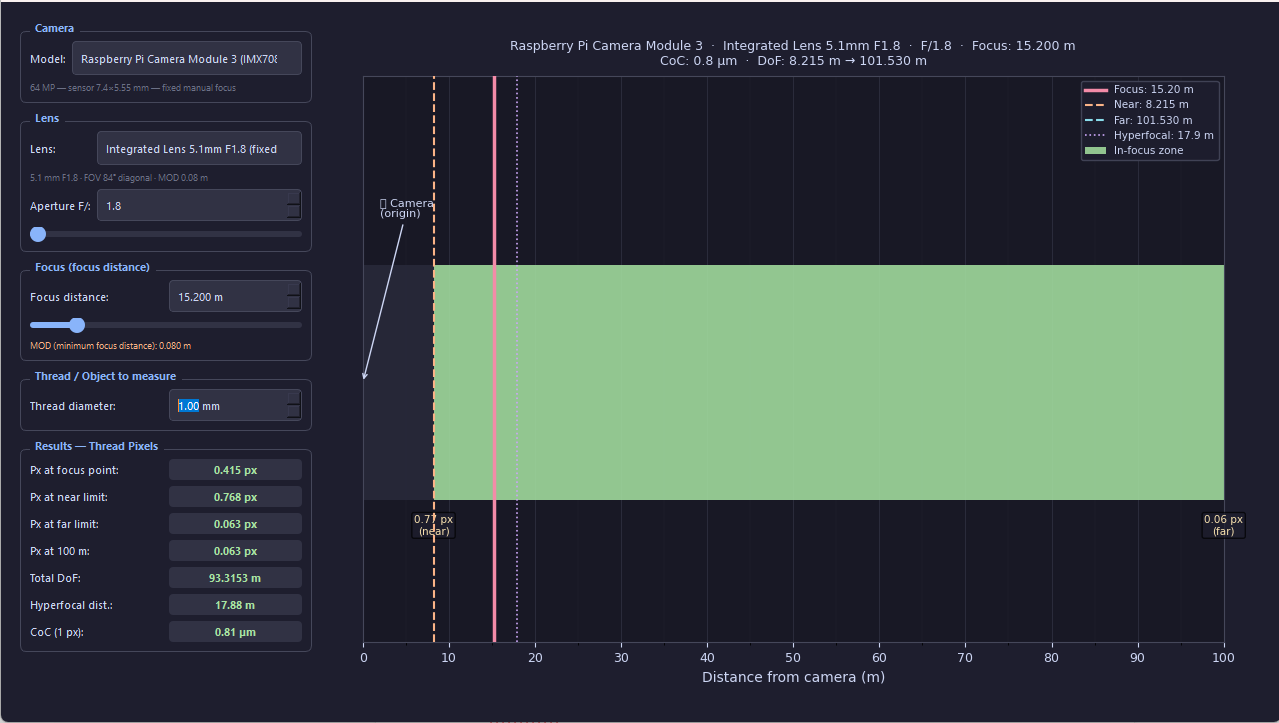
\includegraphics[width=\textwidth]{Images/Figure 3.1.png}
    \caption[Graphical interface of the custom analytical software developed to evaluate the optical performance of the LINKU stereo vision system]{Graphical interface of the custom analytical software developed to evaluate the optical performance of the LINKU stereo vision system. The visualization corresponds to the Hawkeye-based configuration and illustrates the relationship between observation distance, Depth of Field limits, hyperfocal distance, and tether pixel occupancy across the expected operational range of up to 100 m. The interface includes an interactive legend to identify the in-focus region and the transition between geometric and sub-pixel detection regimes.}
    \label{fig:figure3.1}
\end{figure}

The framework also generates comparative visualizations between different optical configurations, enabling rapid evaluation of the trade-off between:

\begin{itemize}
    \item Wide-field situational awareness
    \item Tether geometric localization capability
    \item Long-range radiometric detectability
\end{itemize}

Although the analytical model is based on simplified thin-lens assumptions, it provides a practical first-order estimation of the optical feasibility limits associated with tether observation under the expected mission conditions. The resulting analysis serves as a preliminary design tool for evaluating COTS optical configurations prior to experimental validation.

\section{Orbital illumination physics}

The optical detectability of the tether is strongly influenced by the illumination conditions expected in orbit. Unlike terrestrial environments, where diffuse ambient illumination and textured backgrounds are commonly available, orbital observation is dominated by highly directional solar radiation and extreme radiometric contrast between illuminated objects and deep space.
\\\\
Under these conditions, tether visibility depends not only on geometric resolution, but also on the interaction between the tether surface, solar illumination geometry, and sensor viewing direction. Consequently, understanding the radiometric behavior of thin structures in orbit is essential for evaluating the feasibility of long-range tether detection.

\subsection{Illumination geometry in LEO}

In LEO, the Sun behaves approximately as a collimated illumination source due to its large distance relative to spacecraft dimensions. As a result, incident solar radiation can be modeled as nearly parallel rays across the tethered system.
\\\\
The average solar irradiance near Earth orbit is approximately $E \approx 1360.8 W/m^2$ under standard solar conditions \cite{koppsolar}.
\\\\
This illumination regime differs substantially from terrestrial imaging conditions, where atmospheric scattering and environmental reflections contribute significantly to scene brightness. In orbit, the background is predominantly low-radiance deep space, and radiometric visibility is therefore dominated by direct solar reflection.
\\\\
Consequently, the apparent brightness of the tether depends strongly on:

\begin{itemize}
    \item Solar incidence angle
    \item Observation angle
    \item Tether surface material properties
    \item Local tether orientation relative to the camera line-of-sight
\end{itemize}

Figure \ref{fig:figure3.2} shows the simplified illumination geometry considered for tether observation under orbital-like conditions.

\begin{figure}[!ht]
    \centering
    \begin{minipage}{0.48\textwidth}
        \centering
        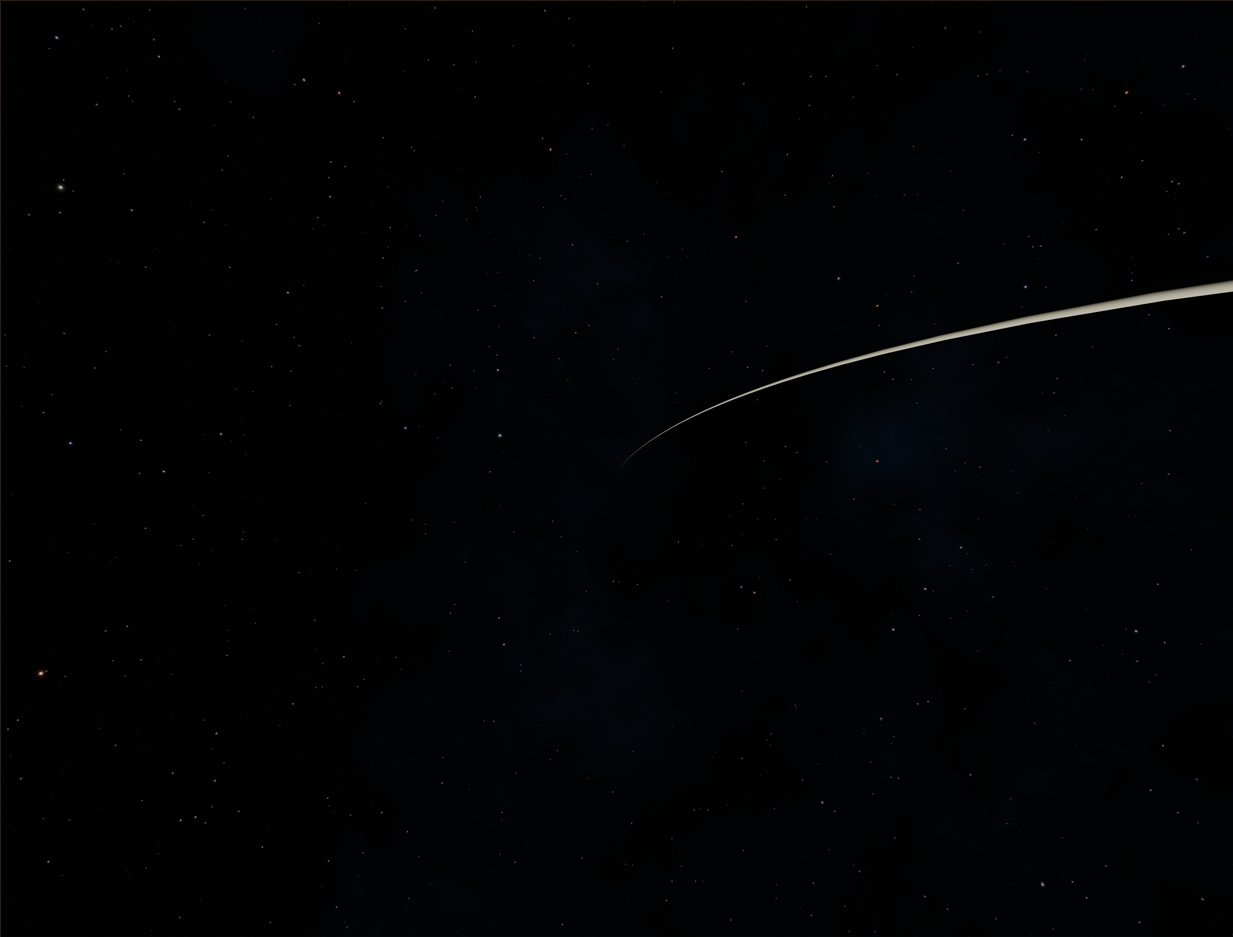
\includegraphics[width=\textwidth]{Images/Figure 3.2a.png}
    \end{minipage}
    \hfill
    \begin{minipage}{0.48\textwidth}
        \centering
        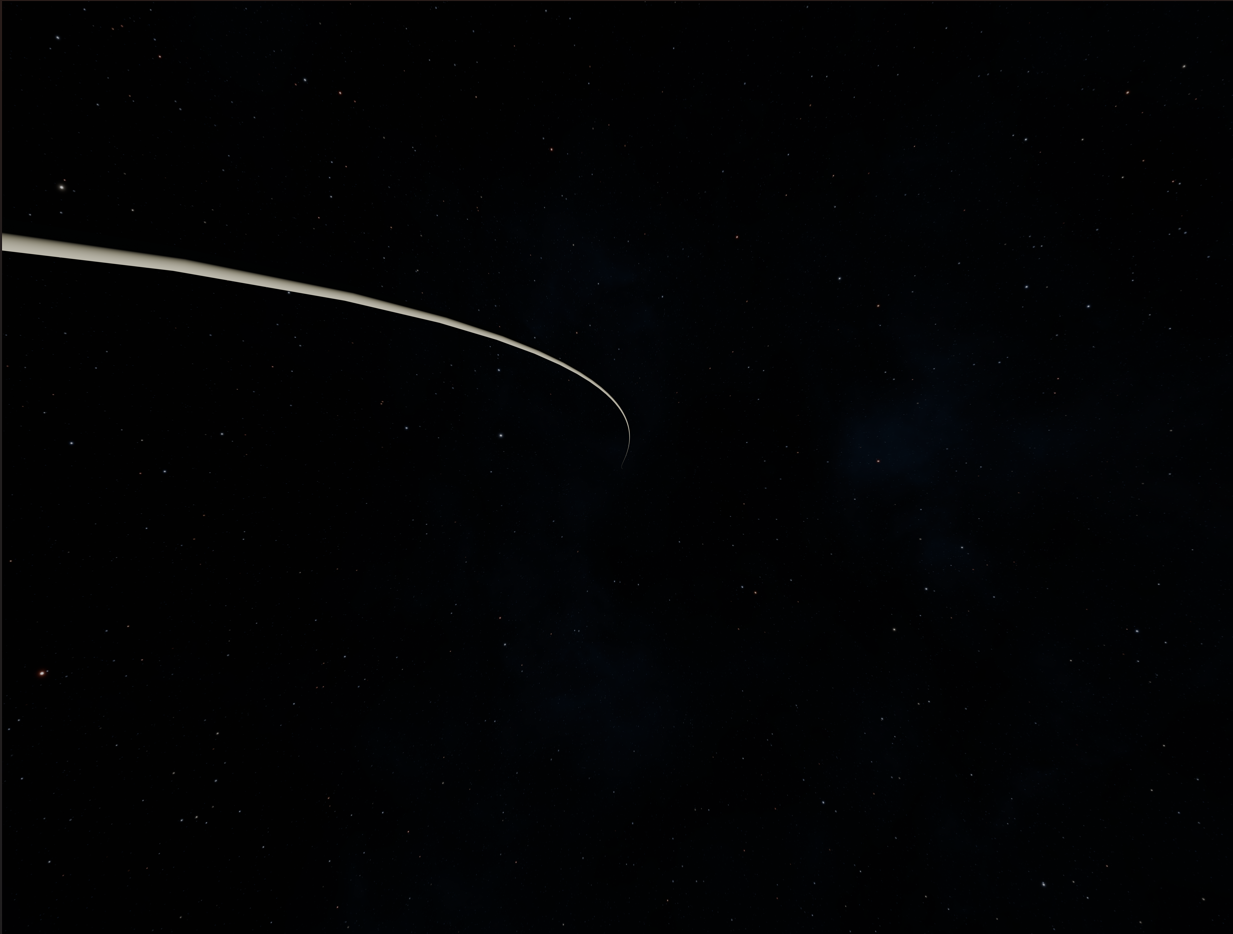
\includegraphics[width=\textwidth]{Images/Figure 3.2b.png}
    \end{minipage}
    \caption[Simulated stereo image pair of the tether under high-contrast orbital-like illumination conditions]{Simulated stereo image pair of the tether under high-contrast orbital-like illumination conditions. The left and right images represent a calibrated stereo pair with identical optical parameters and a fixed baseline of 100 mm. The visualization illustrates the expected appearance of a thin tether against a low-radiance background, highlighting the radiometric contrast and localized brightness variations associated with directional illumination. The figure is intended to represent the expected optical observation conditions rather than a final flight-camera configuration.}
    \label{fig:figure3.2}
\end{figure}

Because the tether diameter is extremely small relative to the observation distance, even minor orientation changes can significantly modify the observed radiometric response. In particular, localized specular reflections may temporarily increase the apparent intensity of the tether against the dark background, enabling detection even when the tether occupies only a fraction of a pixel.

\subsection{Specular reflection and sub-pixel visibility}

At large observation distances, the tether enters the sub-pixel regime described in Section 3.2.3, where direct geometric edge reconstruction becomes increasingly unreliable. Under these conditions, tether visibility depends primarily on radiometric contrast rather than on explicit geometric resolution.
\\\\
If the tether surface exhibits partially specular behavior, incident solar radiation may generate localized reflection peaks observable by the image sensor. These reflections may produce detectable intensity variations even when the projected tether width is substantially smaller than one pixel.
\\\\
This effect becomes particularly relevant under high-contrast orbital conditions because the surrounding background radiance is extremely low. As a result, relatively small reflected signals may become detectable if the sensor dynamic range and exposure conditions are appropriately configured. Figure 3.3 illustrates a conceptual example of stereo tether observation under directional illumination conditions.

\begin{figure}[!ht]
    \centering
    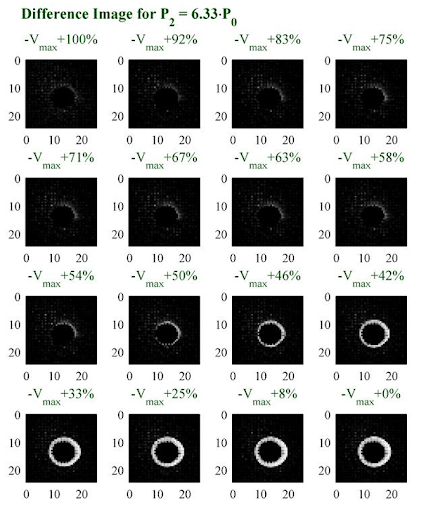
\includegraphics[width=0.75\textwidth]{Images/Figure 3.3.png}
    \caption[Empirical demonstration of blooming across a high-contrast boundary in a CMOS sensor, adapted from Ailuri et al. \cite{ailuri2016blooming}.]{Empirical demonstration of blooming across a high-contrast boundary in a CMOS sensor, adapted from Ailuri et al. \cite{ailuri2016blooming}. The difference image highlights the spatial spreading of charge from the saturated region into adjacent dark pixels, illustrating how radiometric overflow may artificially enlarge the apparent width of thin bright structures under high-contrast illumination conditions.}
    \label{fig:figure3.3}
\end{figure}

However, this visibility mechanism also introduces several challenges:

\begin{itemize}
    \item Reflections may appear intermittently depending on tether orientation
    \item Brightness may vary rapidly along the tether length
    \item Saturation or blooming effects may occur under favorable reflection geometry \cite{ailuri2016blooming, chao2013blooming}
\end{itemize}

Blooming effects in CMOS sensors may spread saturated charge into neighboring pixels, artificially enlarging the apparent width of thin structures and distorting radiometric measurements \cite{ailuri2016blooming}. Consequently, tether detection cannot rely exclusively on stable brightness assumptions. Instead, the reconstruction strategy must tolerate non-uniform radiometric behavior and intermittent visibility conditions.
\\\\
For the present mission concept, blooming is considered only as a possible aid for initial detectability rather than as a reliable geometric measurement mechanism. Saturation-induced charge spreading may increase the apparent footprint of an otherwise sub-pixel tether, facilitating intensity-based detection under high-contrast conditions. However, this apparent width does not represent the true physical diameter of the tether and should not be interpreted as a direct geometric measurement.
\\\\
Under these conditions, accurate reconstruction must rely primarily on radiometric centroiding and stereo geometric constraints rather than on the apparent width of saturated image regions \cite{chao2013blooming, ailuri2016blooming}.
\\\\
These effects further reinforce the limitations of conventional feature-based photogrammetry methods discussed in Chapter 2, since standard correspondence algorithms typically assume relatively stable brightness consistency between stereo views \cite{kniaz2020wire, yu2023bonding}. Figure 3.4 illustrates how bright line-like structures may produce radiometric spreading and blooming artifacts on CMOS image sensors.

\begin{figure}[!ht]
    \centering
    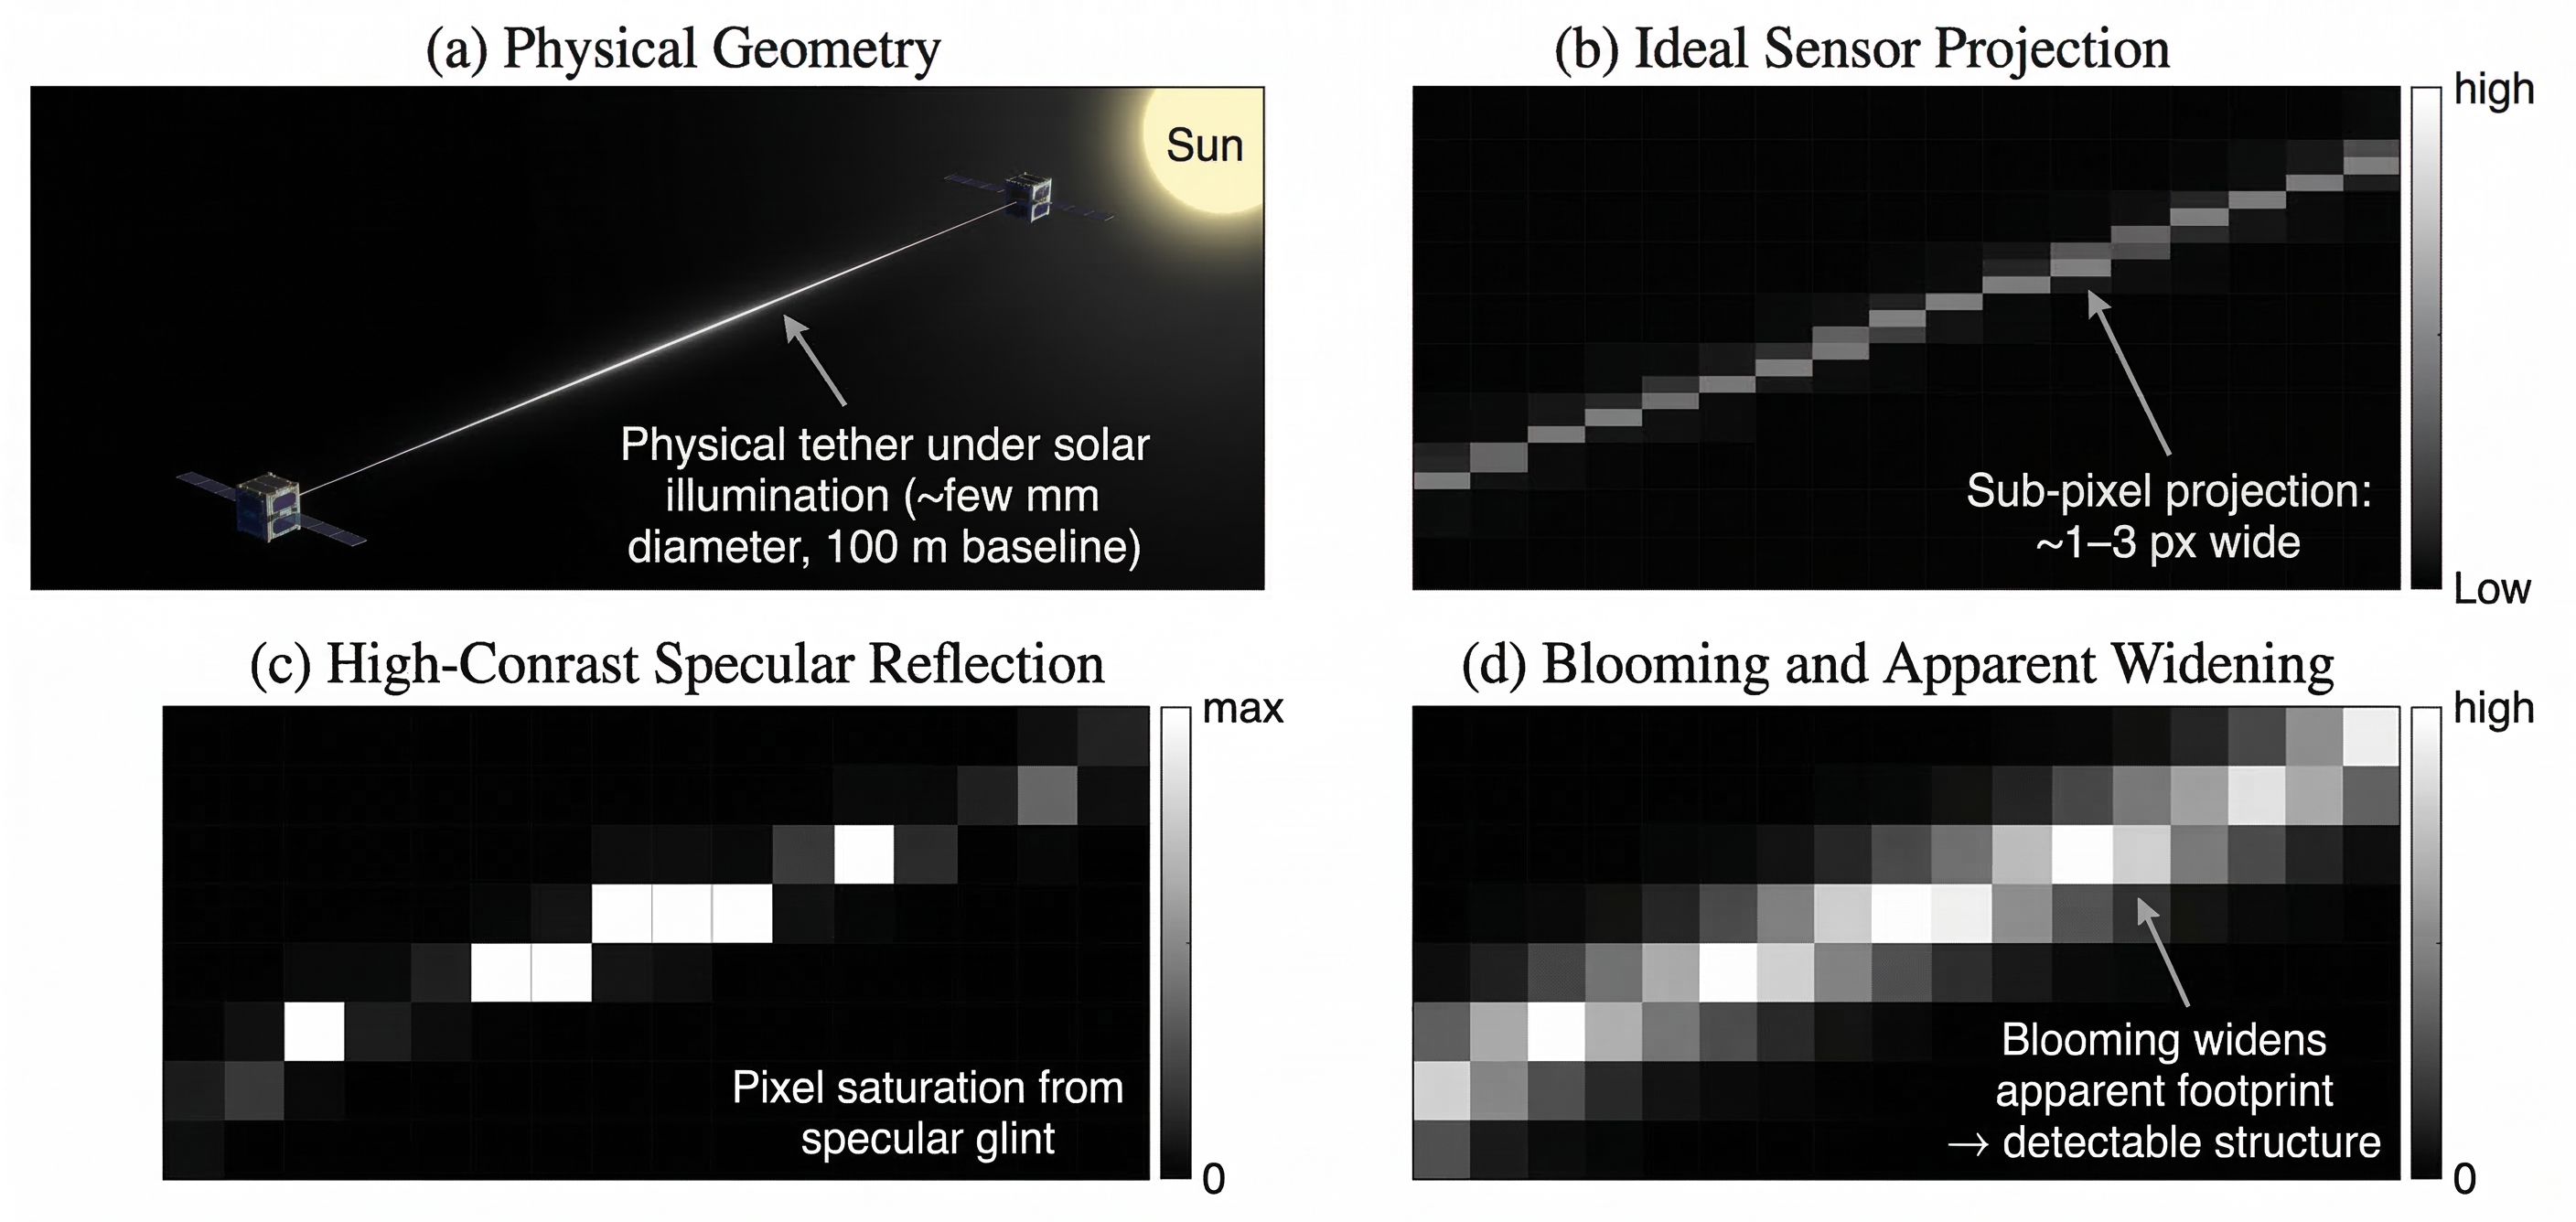
\includegraphics[width=\textwidth]{Images/Figure 3.4.png}
    \caption[Author-generated conceptual illustration of a possible imaging response of a thin tether under high-contrast orbital-like illumination conditions]{Author-generated conceptual illustration of a possible imaging response of a thin tether under high-contrast orbital-like illumination conditions. The figure is intended as an idealized visual aid and does not represent a measured or quantitatively validated blooming width. (a) Simplified physical geometry. (b) Ideal sub-pixel sensor projection. (c) Localized saturation associated with a bright tether response. (d) Qualitative apparent footprint enlargement that may occur due to saturation-induced blooming.}
    \label{fig:figure3.4}
\end{figure}

\subsection{Implications for optical detection strategy}
The orbital illumination conditions analyzed in the previous sections directly influence the reconstruction strategy adopted for the LINKU stereo vision system.
\\\\
As a consequence of the sub-pixel visibility, specular reflection, saturation, and blooming effects discussed above, the optical problem cannot be treated purely as a conventional geometric imaging problem throughout a significant portion of the operational range.
\\\\
Under sub-pixel observation conditions, the tether progressively ceases to be conventionally observable as a fully resolvable geometric object and instead becomes primarily detectable through its radiometric response within the image plane.
\\\\
Due to these conditions, tether detectability depends on a combination of the following:
\\\\
\textbf{Geometric sampling}, which determines the spatial projection of the tether onto the sensor plane.

\begin{figure}[!ht]
    \centering
    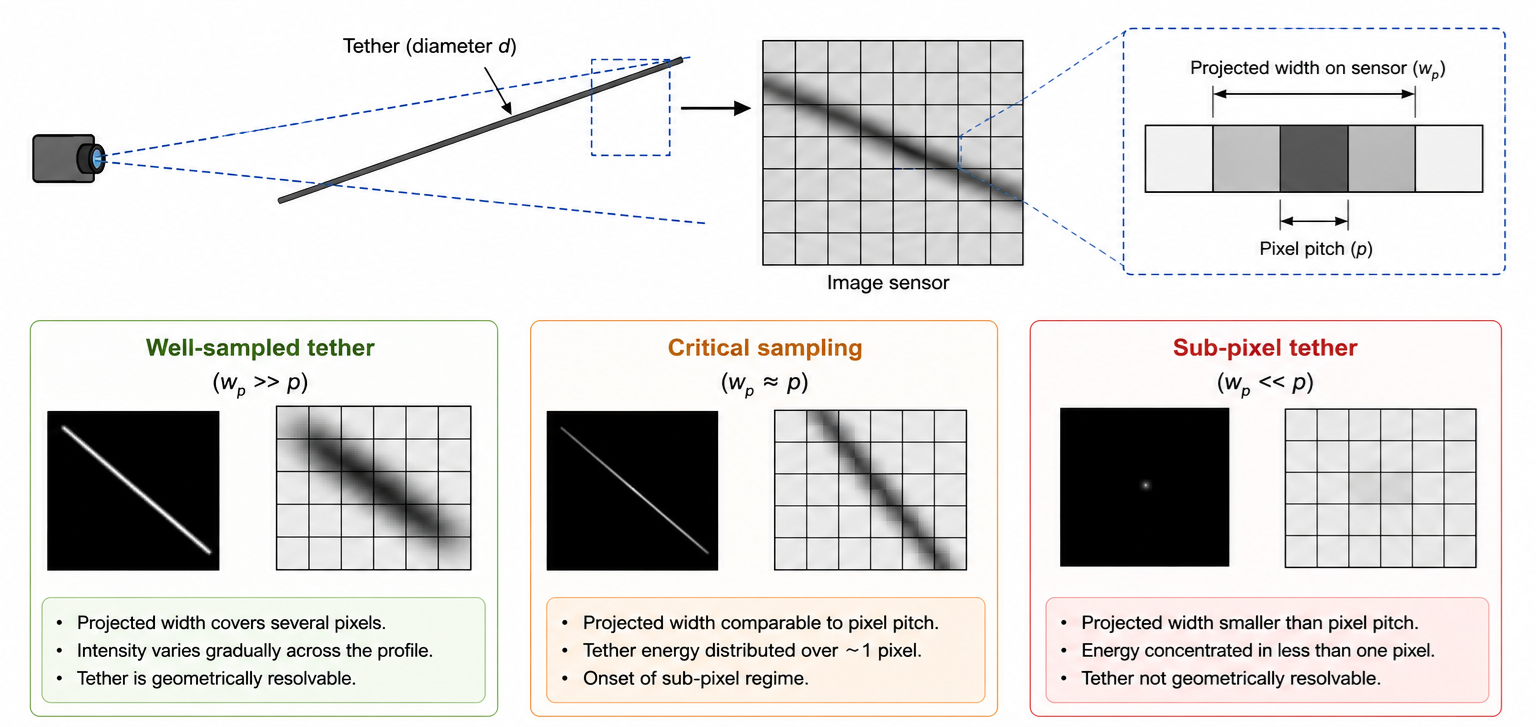
\includegraphics[width=\textwidth]{Images/Figure 3.5.png}
    \caption[Conceptual illustration of the influence of geometric sampling on tether detectability under orbital observation conditions]{Conceptual illustration of the influence of geometric sampling on tether detectability under orbital observation conditions. The figure shows how the tether is projected onto the image sensor and how its apparent width $w_p$ relates to the sensor pixel pitch $p$. Three sampling regimes are presented: well-sampled, critical sampling, and sub-pixel observation. As the projected tether width decreases below the pixel size, the tether progressively loses its directly resolvable geometric structure and becomes primarily observable through its radiometric response. This transition highlights the increasing importance of radiometric-based detection and localization techniques under sub-pixel observation conditions.}
    \label{fig:figure3.5}
\end{figure}

\textbf{Radiometric contrast}, which governs the distinguishability of the tether signal relative to the background.

\begin{figure}[!ht]
    \centering
    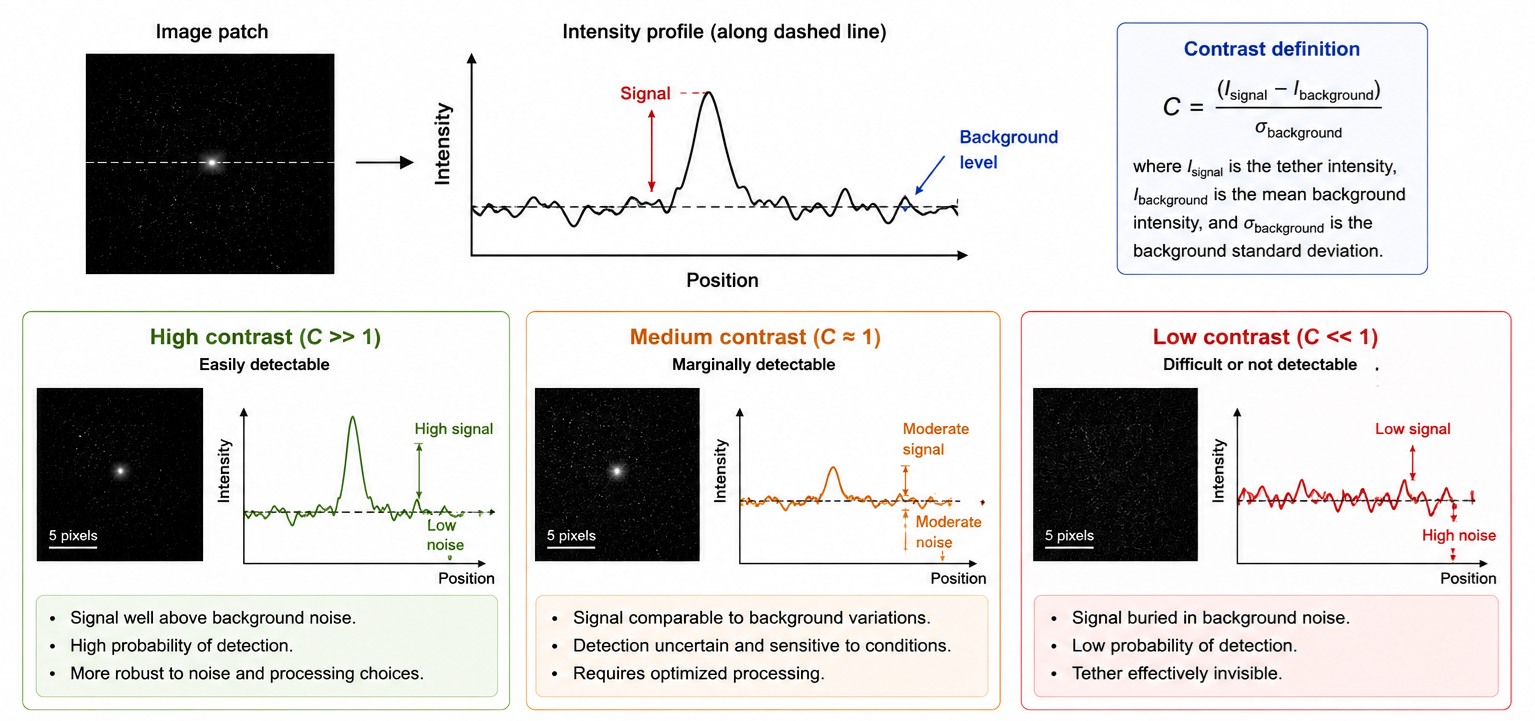
\includegraphics[width=\textwidth]{Images/Figure 3.6.png}
    \caption[Conceptual illustration of the influence of radiometric contrast on tether detectability under sub-pixel orbital observation conditions]{Conceptual illustration of the influence of radiometric contrast on tether detectability under sub-pixel orbital observation conditions. The upper portion of the figure shows the relationship between the tether signal and the surrounding background intensity, highlighting how detectability depends on the signal level relative to background variations and noise. The lower portion presents three representative contrast regimes: high contrast, medium contrast, and low contrast. As radiometric contrast decreases, the tether signal becomes progressively more difficult to distinguish from the background, reducing detection reliability. The figure emphasizes that even when the tether is not geometrically resolvable, it may remain detectable if sufficient radiometric contrast exists between the tether response and the surrounding background. This behavior reinforces the importance of radiometric-based detection and localization techniques under sub-pixel observation conditions.}
    \label{fig:figure3.6}
\end{figure}

\textbf{Directional illumination}, which controls brightness variations through observation geometry and specular reflection effects.

\begin{figure}[!ht]
    \centering
    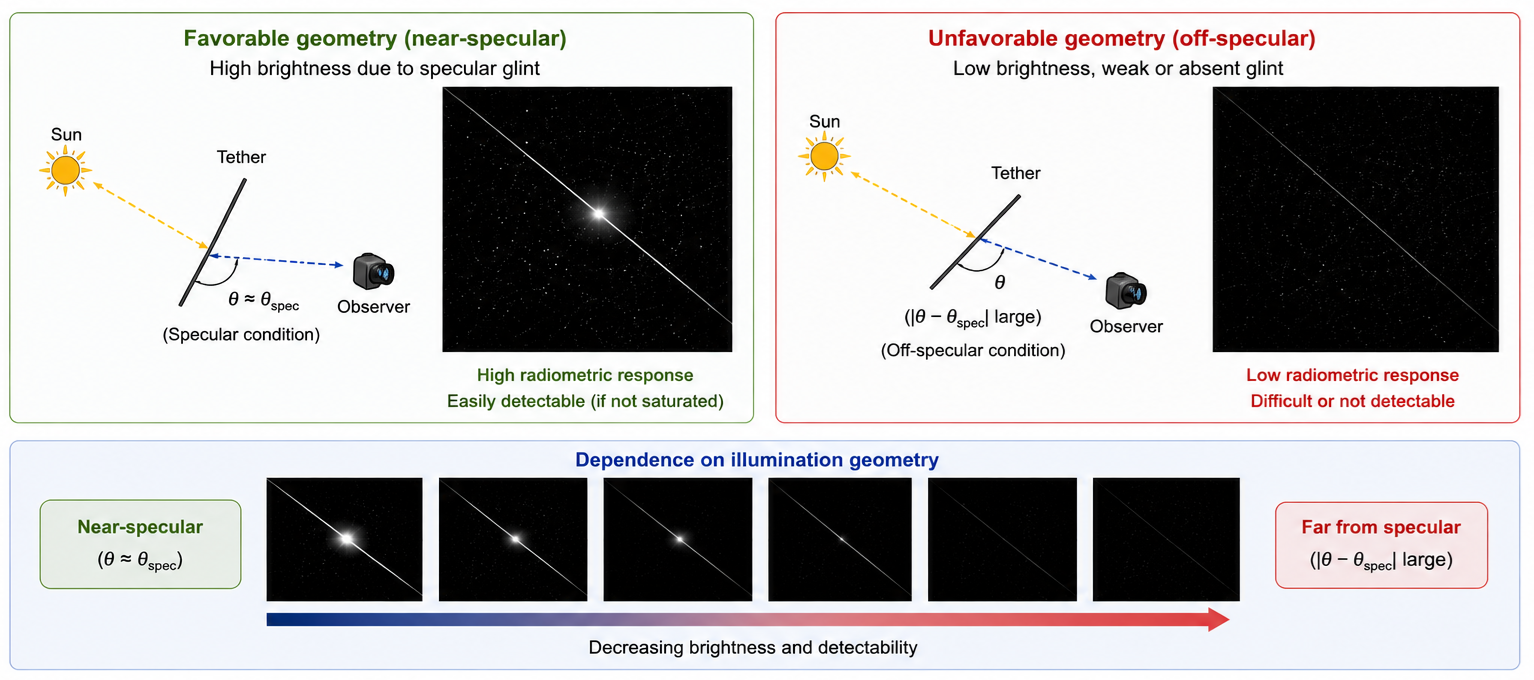
\includegraphics[width=\textwidth]{Images/Figure 3.7.png}
    \caption[Conceptual illustration of the influence of directional illumination on tether detectability under orbital observation conditions]{Conceptual illustration of the influence of directional illumination on tether detectability under orbital observation conditions. The figure shows how the apparent brightness of the tether depends on the relative geometry between the Sun, the tether, and the observer. Under favorable near-specular conditions, reflected sunlight produces a strong radiometric response, increasing tether visibility and detectability. In contrast, under off-specular conditions, the reflected energy reaching the sensor is significantly reduced, resulting in weak radiometric signals and decreased detectability. The lower portion of the figure illustrates the progressive reduction in tether brightness as the observation geometry moves away from the specular reflection condition. This behavior highlights the strong dependence of tether visibility on illumination geometry and explains why a tether may alternate between highly detectable and nearly invisible states despite no change in its physical characteristics.}
    \label{fig:figure3.7}
\end{figure}

\textbf{Temporal visibility conditions}, which introduce intermittent detectability due to orbital motion and changing illumination geometry.

\begin{figure}[!ht]
    \centering
    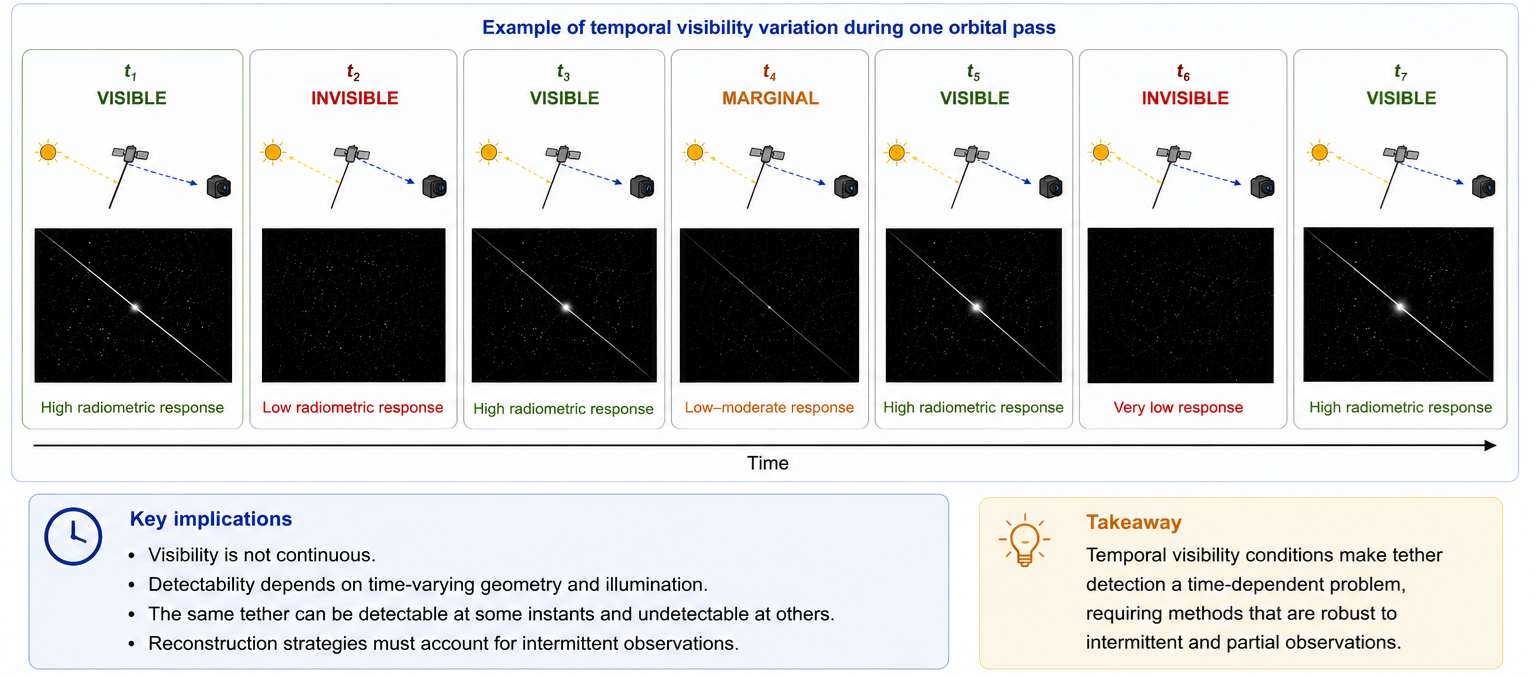
\includegraphics[width=\textwidth]{Images/Figure 3.8.png}
    \caption[Conceptual illustration of temporal visibility effects on tether detectability under orbital observation conditions]{Conceptual illustration of temporal visibility effects on tether detectability under orbital observation conditions. The figure shows how orbital motion, spacecraft attitude variations, and changing Sun--tether--observer geometry can cause the same tether to alternate between visible, marginally visible, and invisible states without any change in its physical properties. This time-dependent radiometric behavior motivates reconstruction strategies capable of operating with partial and intermittently visible observations.}
    \label{fig:figure3.8}
\end{figure}

This motivates the use of geometry-driven reconstruction methods capable of exploiting radiometric signatures, intensity-based extraction, geometric continuity, and stereo correspondence under sub-pixel observation conditions. These methods include:
\begin{itemize}
    \item Centerline estimation
    \item Intensity-based extraction
    \item Geometric curve tracking
    \item Radiometric centroiding
    \item Sub-pixel localization techniques
\end{itemize}

Under these conditions, the apparent tether width produced by saturation-induced blooming should not be interpreted as a direct geometric measurement, reinforcing the need for reconstruction approaches based on radiometric localization and constrained stereo geometry rather than on raw saturated image regions.
\\\\
Additionally, the strong dependency between tether visibility and illumination geometry suggests that experimental validation should incorporate representative high-contrast lighting conditions capable of approximating the directional illumination behavior expected in orbit.
\\\\
For this reason, the experimental design incorporates controlled illumination configurations intended to reproduce the radiometric challenges associated with orbital tether observation.
